\chapter{System Evaluation}

\section{Planning}
At the start of the project, the developer used Jira sprints less strictly than is typical. This strategy caused several issues with work management and progress monitoring, which delayed project completion. After the Christmas break, the developer made the decision to strictly follow the sprint approach, which led to a superior outcome.
It was decided that two-week intervals would be the best size for dividing the sprints. This time frame created a balance between the shortness of a one-week sprint, which might not offer enough time for significant development, and the heavy workload of a sprint lasting longer than two weeks, which might be challenging for the developer to complete in its entirety.
The developer broke down the epics into a number of sub-components, including authentication, dissertation, frontend, backend, and planning, to help with project management. Figure \ref{image:workbreakdown} illustrates how these portions are divided. This divide made it simpler to assign work to team members and monitor progress by helping to identify individual tasks inside each epic.
\begin{figure}[h!]
    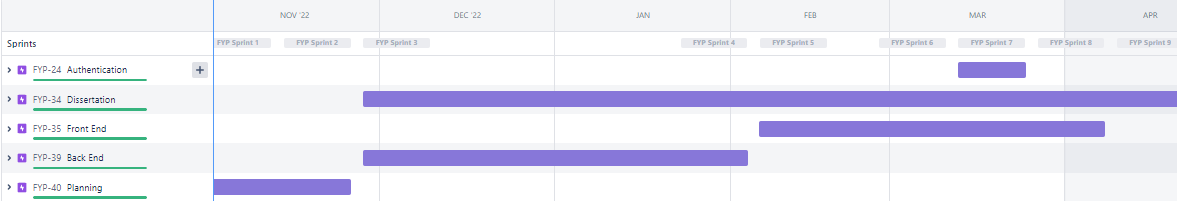
\includegraphics[width=1.0\textwidth]{images/JiraWorkBreakdown.png}
    \centering
    \label{image:workbreakdown}
    \caption{Jira Work Breakdown}
\end{figure}


\section{Testing}
By using Postman to test the backend, the developer was able to properly test the backend functioning, making it simpler to find and fix problems before moving on to the frontend work. This strategy assisted in making sure the backend code was dependable and consistent, which in turn enhanced the application's overall speed.
\newline \newline
The system's backend was tested using Postman, which worked well. The developer was able to manage requests and responses with ease and test the API's different functionalities. In addition, Postman provided a user-friendly interface that made it simple for the developer to write “Automated Tests” to validate the data returned for each of the different API requests. Postmans automated test framework was a big benefit especially as changes were being made to the backend, it was very easy to rerun the automated test suite in postman to make sure that nothing had been broken and if necessary making it simpler to spot any problems and immediately implement fixes.
\newline \newline
Overall, using Postman to test the system's backend was a useful strategy during the application development process. Before beginning frontend development, it enabled the developer to extensively test the backend code and guarantee the overall quality and dependability of the system. The system became stronger and functioned better as a result, which eventually benefited the end users.
\newline \newline


\section{Application}
The method for filing invoices was tested by the developer, who discovered that it worked well overall. The solution seemed to be relevant for small businesses that needed to track their payment and invoicing processes.
\newline \newline
However, upon closer examination, the developer found that they did not make full use of the folder and company backend components. In retrospect, the developer recommendations for future development to include a dropdown list with all potential company names as possibilities in the name input box when submitting a new invoice. A simpler and more efficient invoices procedure would be possible as a result.
\newline \newline
Additionally, the developer recommends creating a company screen where users can view all companies and select them to see all related invoices. This would provide a more organised and user-friendly approach to managing invoicing and payments for multiple companies.
\newline \newline
From a usability point of view it might be beneficial to have a summary / dashboard like screen which showed high level information/ metrics such as the following:
\begin{itemize}
    \item Total Money Due Overall
    \item Total Money Due in Next 7 Days - and if applicable, a button that the user can click to go directly to that specific list of invoices.
    \item Total Money Overdue - with a button that the user can click to go directly to the list of overdue invoices and take action on them
\end{itemize}


\section{Objectives}
The initial objectives of this project was to design and develop an application that facilitated effortless storage of invoices for the end users by offering a user-friendly interface. The project would offer suggestions for improvement in various sections of the application.

\subsection{Were the objectives met?}
Given the limitations of the developer's ability, time, and effort, the project's objectives were successfully met to the greatest extent possible. Despite this, there are still certain things that could be done better, like improving the application's quality. It is stated that the developer's current resources and capabilities place a cap on these advancements. However, the goals that were reached meet the essential requirements and provide a solid groundwork for future progress.

\subsection{Where the objectives were met}

\begin{itemize}
    \item The application successfully eliminates the need for excessive paper documentation and simplifies the process of tracking invoices
    \item The developer learnt how to use React Native effectively and now feels confident to apply it in future application development.
    \item The developer increased their knowledge of JavaScript programming language
\end{itemize}


